\section{File HTML}

\begin{figure}[h]
    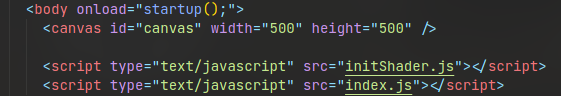
\includegraphics[width= \textwidth]{grafika/html.png}
    \caption{file html yang digunakan}
    \label{fig:html}
\end{figure}

seperti yang bisa dilihat dalam gambar \ref{fig:html}, file html ini akan berfungsi untuk mengatur ukuran dari canvas yang akan digunakan.
Canvas sendiri adalah tempat dimana webgl bisa melakukan manipulasi piksel secara bebas

selain itu, juga dilakukan import \emph{script initShader.js} dan \emph{index.js}.
\emph{initShader.js} digunakan untuk melakukan inisiasi Vertex Shader dan Fragment Shader.
sedangkan \emph{index.js} berisi program utama.



\section{initShader.js}

\subsection{loadShader}

\begin{figure}[h]
    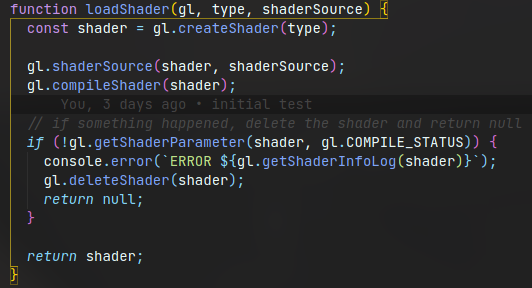
\includegraphics[width = \textwidth]{grafika/loadShader.png}
    \caption{fungsi \emph{loadShader} dalam \emph{initShader.js}}
    \label{fig: loadShader}
\end{figure}

fungsi dalam gambar \ref{fig: loadShader} digunakan untuk melakukan
kompilasi terhadap shader yang digunakan. Hasil dari kompilasi akan
digunakan untuk mengatur bagaimana sebuah vertex akan ditampilkan
di dalam canvas. Apabila dalam proses kompilasi terjadi error, maka
shader yang sudah dikompilasi tadi akan dihapus dan fungsi akan melakukan
return null.

\subsection{setupShader}

\begin{figure}[h]
    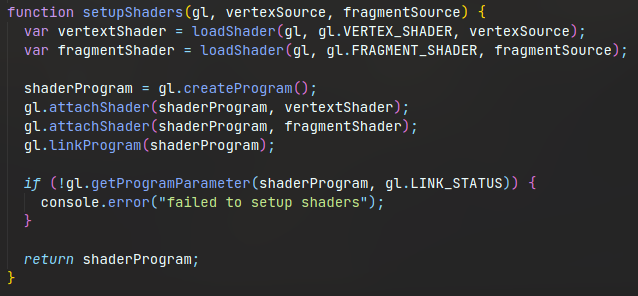
\includegraphics[width=\textwidth]{grafika/setupShader.png}
    \caption{fungsi setupShader dalam initShader.js}
    \label{fig: setupShader}
\end{figure}

setiap program webgl akan memerlukan vertex shader dan fragment shader.
program di gambar \ref{fig: setupShader} digunakan untuk menggabungkan
antara vertex shader dan fragment shader dan dengan menggunakan \emph{linkProgram} menghubungkan antara program
dengan shader yang sudah digabung tadi.



\section{index.js}

\subsection{setup vertexShader}

\begin{figure}[h]
    \centering
    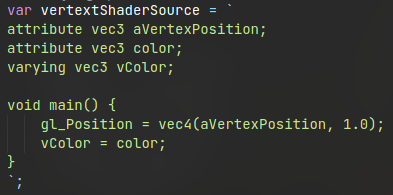
\includegraphics{grafika/vertexShader.png}
    \caption{vertexShader}
    \label{fig: vertexShader}
\end{figure}

yang pertama kali harus di set dalam program webgl adalah vertex shader dan fragment shader.
dalam vertex Shader, harus terdapat fungsi main, yaitu fungsi yang pertama kali akan dipanggil
oleh webgl. Selain itu, juga harus terdapat assign value ke gl\_Position yang akan digunakan oleh
webgl untuk mengetahui posisi piksel yang akan digambar.

hal lain yang harus dilihat adalah \emph{attribute} dan \emph{varying} yang terdapat dalam program vertex.
\emph{attribute} digunakan untuk menghubungkan antara program (dalam hal ini index.js) dengan shader. sedangkan
\emph{varying} digunakan untuk menghubungkan antara vertex Shader dengan fragment Shader. Terdapat satu lagi jenis variabel
yang tidak dipakai dalam shader ini adalah \emph{uniform}.

untuk saat ini, dalam vertex Shader kita hanya melakukan assign gl\_Position dan vColor.

\subsection{setup fragmentShader}

\begin{figure}[h]
    \centering
    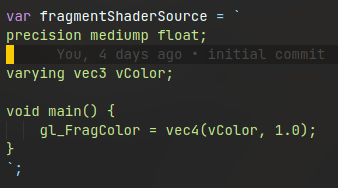
\includegraphics{grafika/fragment shader.png}
    \caption{fragmentShader}
    \label{fig: fragmentShader}
\end{figure}

fragment shader berguna untuk melakukan set bagaimana warna dari suatu vertex.
dalam gambar \ref{fig: fragmentShader}, kita hanya mengambil value yang di set di vertex Shader dan memasukkannya ke dalam gl\_FragColor.
gl\_FragColor digunakan oleh webgl dan harus ada dalam fragment Shader.

\subsection{create WebGL Context}


\begin{figure}[h]
    \centering
    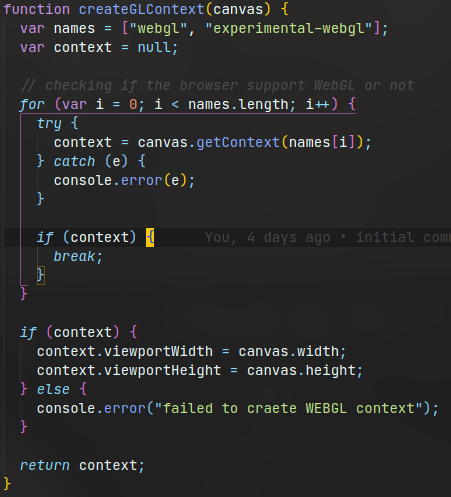
\includegraphics{grafika/createContext.png}
    \caption{fungsi createContext}
    \label{fig: createContext}
\end{figure}

sebelum melakukan proses gambar dengan menggunakan webgl, kita memerlukan context webGL terlebih dahulu.
secara general, kita hanya tinggal memanggil fungsi \emph{getContext}, namun terdapat beberapa browser yang tidak
memiliki support webGL secara default.

fungsi di gambar \ref{fig: createContext} secara otomatis memilih backend webgl, apakah itu webgl atau experimental-webgl.
context ini nantinya akan digunakan dalam seluruh program.

\subsection{fungsi Draw}


\begin{figure}[h]
    \centering
    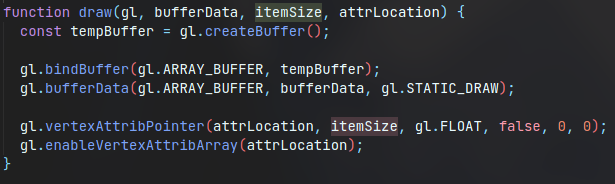
\includegraphics[width=\textwidth]{grafika/draw.png}
    \caption{fungsi draw}
    \label{fig: draw}
\end{figure}

fungsi draw ini digunakan untuk melakukan assign terhadap attribute - attribute yang sudah ditulis baik di
vertex Shader maupun fragment Shader. dalam WebGl, buffer hanya dapat menyimpan 1 variabel saja, sehingga apabila
terdapat 2 attribute atau lebih kita harus melakukan bindBuffer lagi.

dalam gambar \ref{fig: draw}, dilakukan inisialisasi buffer kosong dan melakukan bind terhadapt buffer kosong tersebut
ke dalam internal variabel webGL. Untuk mengisi variabel yang sudah di bind tersebut, kita menggunakan fungsi \emph{bufferData}.
di dalam fungsi tersebut, selain melakukan assign data ke buffer, kita juga harus mengatur bagaimana penggunaan variabel tersebut,
untuk saat ini menggunakan konstanta gl.STATIC\_DRAW yang berarti variabel tersebut di set sekali dan digunakan berkali - kali.

selanjutnya, dilakukan assign variabel tersebut ke dalam vertex Shader dengan menggunakan fungsi \emph{vertexAttribPointer} dan dilakukan
enable terhadap fungsi tersebut menggunakan \emph{enableVertexAttribArray}.

\subsection{fungsi Startup}

\begin{figure}[!h]
    \centering
    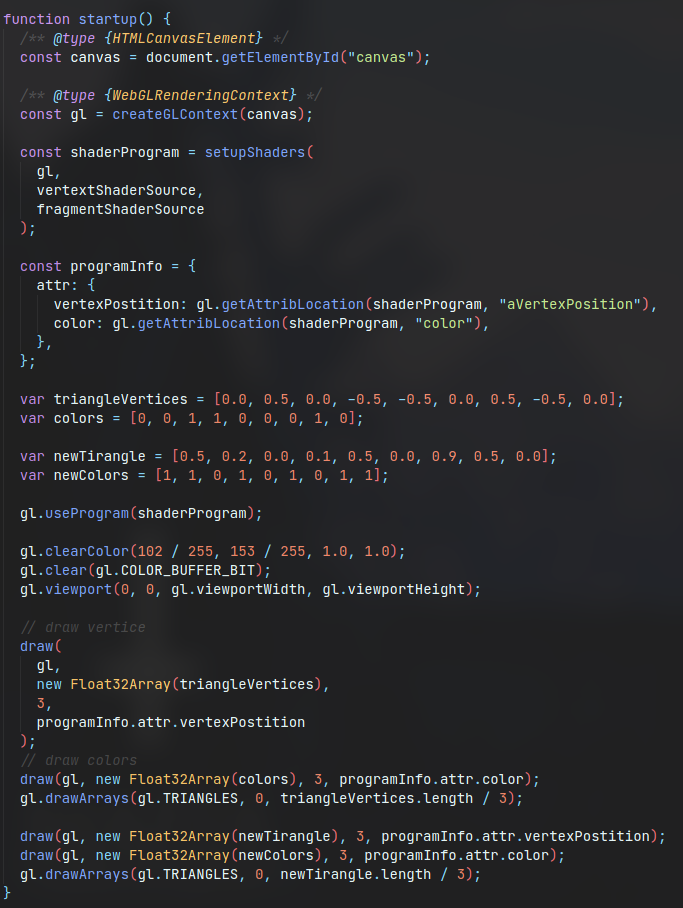
\includegraphics[width=\textwidth]{grafika/startup.png}
    \caption{fungsi startup}
    \label{fig: startup}
\end{figure}

fungsi ini adalah fungsi yang pertama kali dipanggil saat page sudah diload. Seperti bisa dilihat pada gambar \ref{fig: startup},
pada bagian pertama kita membuat context dengan fungsi yang sudah ditulis diatas. Selanjutnya mengatur shader yang digunakan
dan menyimpan value attribute shader kedalam variabel. \emph{useProgram} digunakan untuk memilih shaderProgram yang mana yang akan
digunakan oleh program saat ini.

Untuk menggambar segitiga, kita harus mengetahui koordinat dari webGL, yaitu pada pojok kiri atas memiliki koordinat (-1,1),
pojok kanan atas (1,1) dan seterusnya dengan koordinat (0,0) berada di tengah - tengah. Sedangkan untuk melakukan assign warna,
perlu diketahui bahwa warna di WebGl menggunakan float antara 0 - 1.

Hal lain yang harus kita lakukan sebelum mulai menggambar segitiga adalah mengatur warna background, diatur menggunakan fungsi
\emph{clearColor}. Selain itu, juga perlu mengatur berapa ukuran viewport atau dalam hal ini canvas yang dipakai oleh webGL.

Setelah memanggil fungsi draw yang sudah dibuat diatas, kita hanya tinggal memanggil \emph{drawArrays}. \emph{drawArrays} akan
menggambar berdasarkan value - value yang sudah di set pada saat memanggil fungsi draw. Perlu dilihat bahwa untuk saat ini kita
menggunakan konstanta \emph{gl.TRIANGLES} karena hanya perlu menggambar segitiga saja, untuk menggambar objek lain mungkin akan
menggunakan konstanta yag lain.

Apabila ingin menggambar beberapa objek sekaligus dengan shader yang sama, kita hanya perlu memanggil fungsi draw dan drawArrays lagi
maka  objek - objek tersebut akan ditampilkan di dalam canvas.

\section*{Catatan}
seluruh kode dalam laporan ini dapat diakses pada url \url{https://github.com/chillytaka/webGL} \\
demo untuk project ini dapat diakses pada url \url{https://chillytaka.github.io/webgl-1}



